
\iffalse 
Assignment 6B
Date    : 11th May 2021
Course  : Applied Programming Lab(EE2703)
Faculty : Prof. Harishankar Ramachandhran

Submission by : Santosh G (EE19B055)

To compile and get the Report(PDF):
1) python3 EE2703_ASSIGN6B_EE19B055.py  (Atleast Once, for the plots)
2) pdflatex EE2703_ASSIGN6B_EE19B055.tex
 
PS: Run "EE2703_ASSIGN6B_EE19B055.py" using the above command atleast once before running this code, as this program needs the plots.
\fi
\documentclass[11pt, a4paper]{article}
\usepackage{graphicx}
\usepackage{amsmath}
\usepackage[margin=0.6in]{geometry}
\usepackage{listings}
\usepackage{float}
\usepackage{mathtools}
\usepackage[thinc]{esdiff}

\title{APL(EE2703): The Laplace Transform(Assignment 6B)} % Title
\author{Santosh G  (EE19B055)} % Author name
\date{\today} % Date for the report

\begin{document}
    \maketitle % Insert the title, author and date

    \section{Aim of the Assignment:}   %Introduction to the assignment
        \begin{itemize}
            \item Analyse LTI systems using Laplace Tranformations
            \item Use SciPy Signals toolkit in Python for the above
            \item Plot various graphs and draw conclusions from them.
        \end{itemize}
        
    \section{Introduction}
    Signals Toolkit of the Scientific Python(SciPy) is very useful to anayse signals, Linear Time Invariant Systems, Circuits and multiple other things, in this assignment we shall use the toolbox to do the the laplace transofrmation and solve the questions. Laplace Transformation changes equation etc from time domain to laplace domain simplyfing the questions that are to be solved and analysis of the same becomes easier.
       
        \section{Questions}
        \subsection{Questions 1, 2 : Varying Decay constant}
    	We use the Laplace transform to solve a simple spring system. The system is characterized by the given differential equation. 
    	\begin{equation}
    		\ddot{x} + 2.25x = f(t) 
    	\end{equation}
    	
    	
    	when considered in the laplace domain, the equation transforms into
    	\begin{equation}
    	  X(s) =  \frac{F(s)}{s^2+2.25}
    	\end{equation}

	The F(s) is of the input signal f(t) which is of the form "\(\cos{(\omega t)}\exp(-at)u(t)\)", where a is the decay factor and $\omega$ is the frequency of the cosine.\\
\\The Laplace Transform of the such input signal f(t) is given by\\ \[ F(s) = \frac{s+a}{(s+a)^2+\omega^2 }\]\\ These polynomials are defined using "poly1d" which are then multiplied to get the output laplace transform. Finally we take the Inverse Laplace Transform of the function using "sp.impulse" to get the time domain sequences and those are plotted. We do this for the natural frequency of the system $\omega$=1.5, and decay values of "a" as 0.5 and 0.05.\\
    	
    	\pagebreak
	The following plots are obtained after solving the above.\\
	\\Plots:
	       \begin{figure}[H]
                    \centering
                    \setlength\tabcolsep{2pt}
                    \begin{tabular}{cc}
                       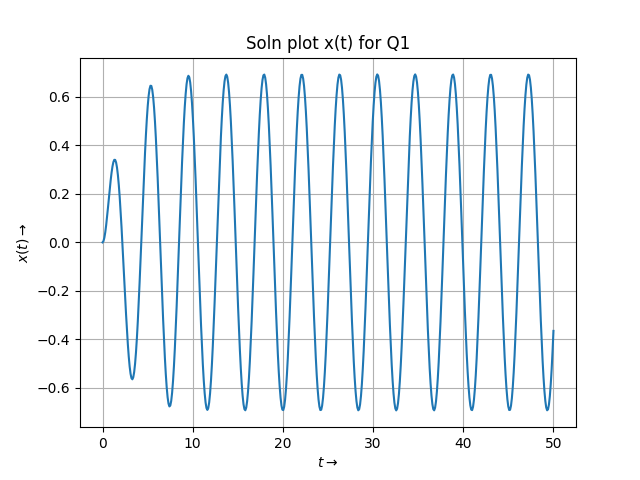
\includegraphics[scale=0.9]{Figure 1.png}
                    \end{tabular}
                    \caption{x(t) with decay constant "a" as 0.5} 
                \end{figure}
                \begin{figure}[H]
                    \centering
                    \setlength\tabcolsep{2pt}
                    \begin{tabular}{cc}
                       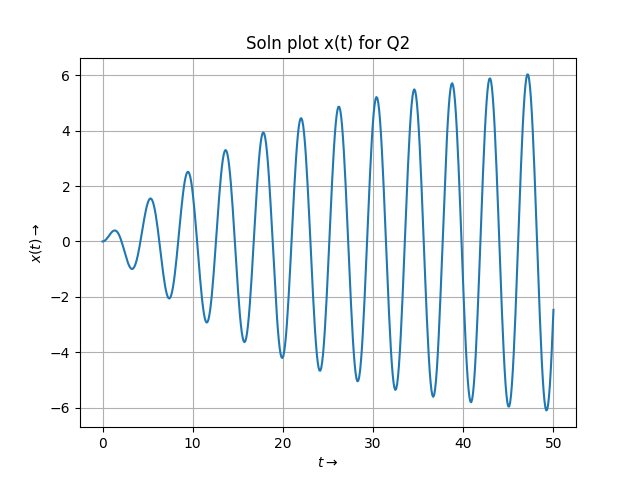
\includegraphics[scale=0.9]{Figure 2.png}
                    \end{tabular}
                    \caption{x(t) with decay constant "a" as 0.05} 
                \end{figure}
	 \pagebreak
	 
	 Following observations are made:	
            \begin{itemize}
	    \item
	    x(t) has a higher amplitude when f(t) has lower decay contstant 
	    \item
	    x(t) takes more time to saturate in case of a lower decay constant, as the resistance offered is less
	    \item
	    Amplitude of x(t) converges to a fixed value in both the cases
	    \end{itemize}
    				
        \subsection{Question 3 : Varying Input Frequency}
 	
    	Let the Transfer function H(s) be of the for as shown below:
    	\begin{equation}
    	  H(s) =  \frac{X(s)}{F(s)} = \frac{((s+a)^2+\omega^2)}{(s^2+2.25)(s+a)}
    	\end{equation}

	where "a" varies from 1.4 to 1.6.
	The following plot is obtained after considering the above frequencies.\\
	\\Plots:
	       \begin{figure}[H]
                    \centering
                    \setlength\tabcolsep{2pt}
                    \begin{tabular}{cc}
                       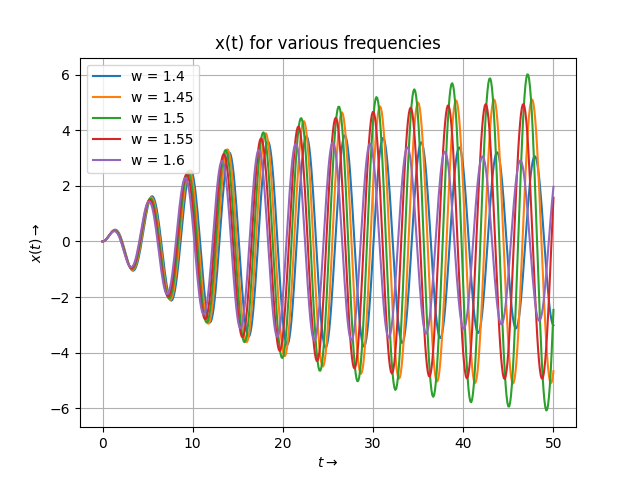
\includegraphics[scale=0.9]{Figure 3.png}
                    \end{tabular}
                    \caption{x(t) with varying input frequencies} 
                \end{figure}

	    By virtue of resonance, when input frequency matches the natural frequency of the system the particular output has the highest amplitude among the other cases.
	  
	\subsection{Question 4 : Coupled Mass system}
 	
    	In this problem we have the two following differential equations and two variables to solve for:\\
    	\[\ddot{x} + (x-y) = 0 \]
	\[\ddot{y} + 2(y-x) = 0 \]
	On trying to solve the equations we get a fourth order differential equation in terms of x. Simplifying by assuming the initial condition x(0) = 1; and substituting to find the equation we would get the following results:\\
	\[X(s) = \frac{s^2+2}{s^3+3s} \]\\
	\[Y(s) =  \frac{2}{s^3+3s} \]\\
        
        We can hence find the time domain series by taking the Inverse Laplace Transform of the above.
        \\By solving the above we obatin the following results which are plotted as shown.\\
        \\Plots:
	       \begin{figure}[H]
                    \centering
                    \setlength\tabcolsep{2pt}
                    \begin{tabular}{cc}
                       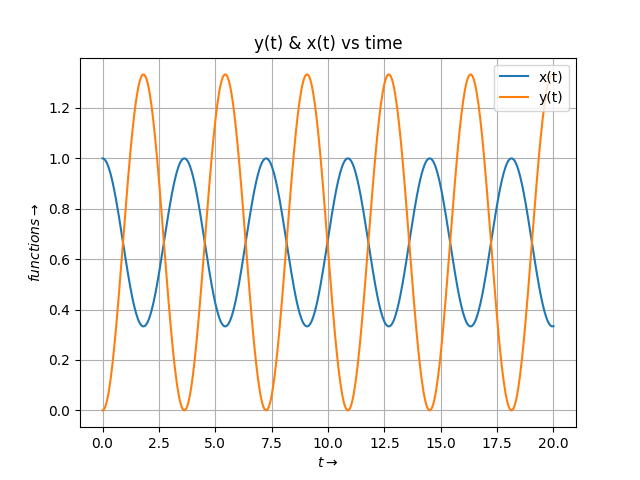
\includegraphics[scale=0.9]{Figure 4.png}
                    \end{tabular}
                    \caption{Plots of x(t) and y(t) vs time} 
                \end{figure}
         \begin{itemize}
         \item
         The functions are opposite in phase(i.e have a phase difference of 180 degrees)
         \item
         This model can be compared to coupled spring mass system.
         
         \end{itemize}

	\subsection{Questions 5, 6 : LCR Filter}
 	
    	On finding the transfer function in the given circuit, we find the following result:\\
	\begin{equation}
        \frac{V_o(s)}{V_i(s)} = \mathcal{H}(s) = \frac{10^6}{s^2+100s+10^6}
    \end{equation}
	and the input is of the form
	\[x(t) = \cos{(10^3t)}+\cos{(10^6t)} \]\\
        
       It is clear that the input is a superposition of two sinusoids with large variance in frequencies.\\
       
       Firstly the bode plots are plotted, in which magnitude and phase are shown in the following:
	       \begin{figure}[H]
                    \centering
                    \setlength\tabcolsep{2pt}
                    \begin{tabular}{cc}
                       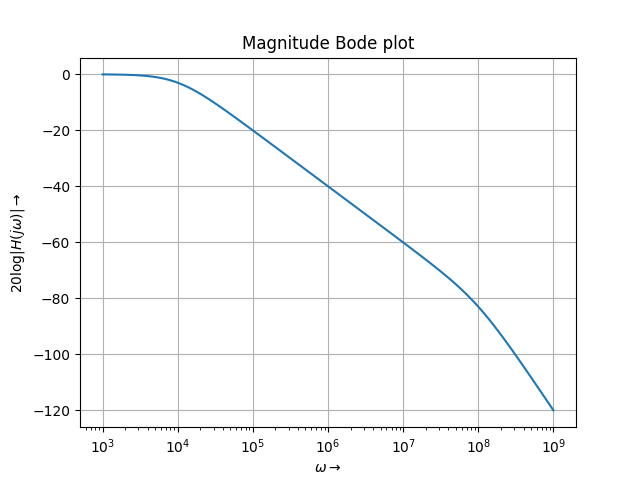
\includegraphics[scale=0.9]{Figure 5a.png}
                    \end{tabular}
                    \caption{Magnitude Bode Plot of the Transfer Function} 
                \end{figure}
	       \begin{figure}[H]
                    \centering
                    \setlength\tabcolsep{2pt}
                    \begin{tabular}{cc}
                       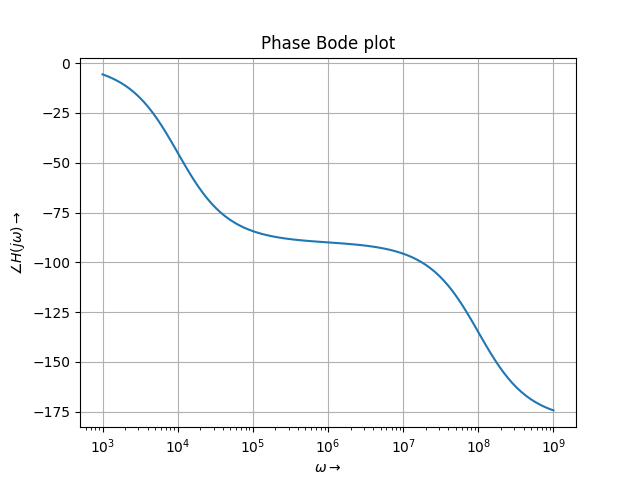
\includegraphics[scale=0.9]{Figure 5b.png}
                    \end{tabular}
                    \caption{Phase Bode Plot of the Transfer Function} 
                \end{figure}
                \pagebreak
                
       Now the ouputs are plotted over various time intervals. One plot shall be plotted in the interval 0 to 30$\mu$s(i.e short term response). Second plot shall be plotted in the interval 0 to 25 msec(i.e long term response). As the frequencies in the order $10^3$  and $10^6$ , considering intervals of microseconds and milliseconds would be useful to analyse the circuit and the transfer function.\\
       
       The plot of output voltage in long time interval is as shown below:
      		  \begin{figure}[H]
                    \centering
                    \setlength\tabcolsep{2pt}
                    \begin{tabular}{cc}
                       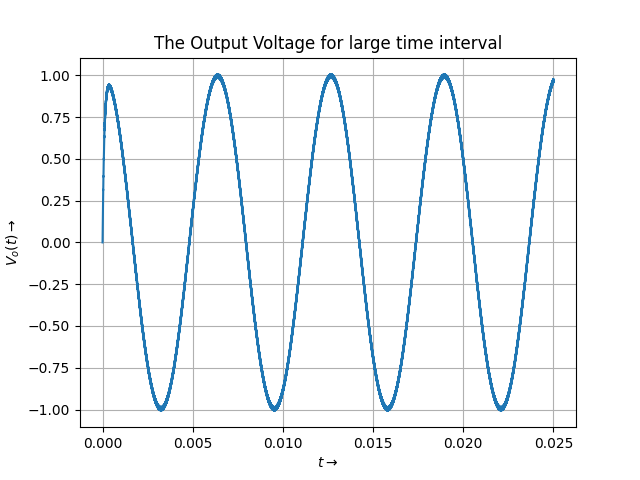
\includegraphics[scale=0.81]{Figure 6a.png}
                    \end{tabular}
                    \caption{Output voltage plot over long interval} 
                \end{figure}
       
              The plot of output voltage in short time interval is as shown below:
      		  \begin{figure}[H]
                    \centering
                    \setlength\tabcolsep{2pt}
                    \begin{tabular}{cc}
                       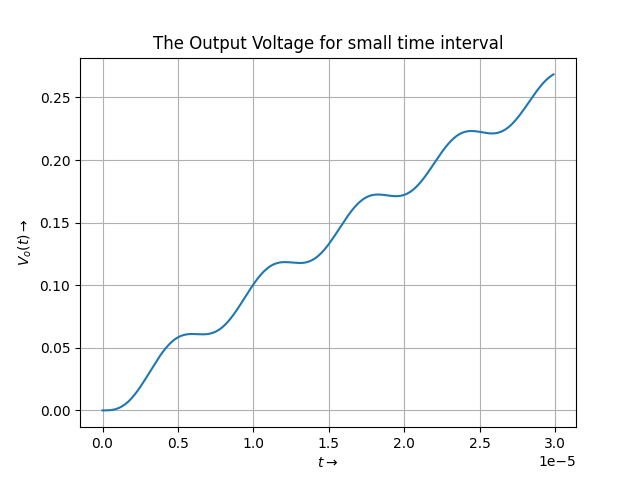
\includegraphics[scale=0.85]{Figure 6b.png}
                    \end{tabular}
                    \caption{Output voltage plot over short interval} 
                \end{figure}
    
   		\begin{itemize}
   		\item 
   		As the magnitude bode plot is monotonically decreasing as frequency increases, it is a low pass filter and we can see two poles from the phase plot, hence the transfer is a 2nd Order Low Pass filter
		\item
		In the short interval plot, the high frequency term($10^6$) can be seen as ripple terms, due to its very high frequency it fails to appear in the long interval plot.
		\item
		The low frequency component($10^3$) passes almost as it is, whereas the high frequency component($10^6$) is attenuated and fails to appear significantly in the final plot, making it clear, that this system is a low pass filter and also because the lower frequency lies within the 3dB bandwidth of the system.

		\end{itemize}

    \section{Conclusion}
    \begin{itemize}
    \item
    We have analyzed Laplace Transformation using Signals Toolbox of Python, which has quite a many inbuilt functions to make the processing much easier, to sketch Bode Plots, find Impulse response, Compute ILTs etc
    
    \item
    RLC Circuit can be used to realise a Low Pass filter, by considering the voltage across the capacitor     
    \end{itemize}    
\end{document}
